\begin{frame}{Noise estimation}{Data}
\begin{columns}
\begin{column}{8cm}
\begin{figure}[H]
		\label{data_2d}\caption{Data in 2D}
		\centering
    	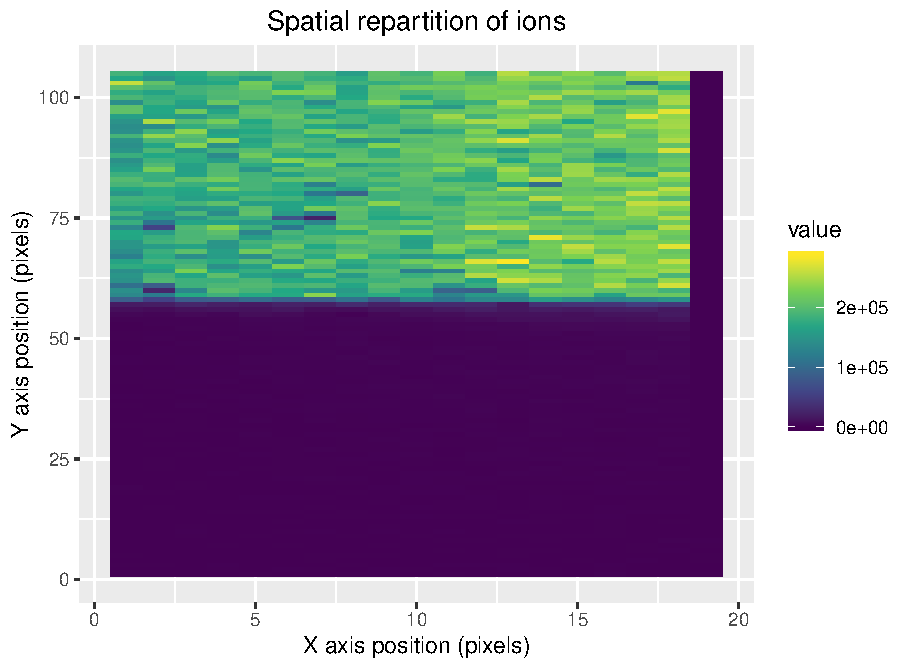
\includegraphics[scale = .5, keepaspectratio]{application/response_estimation/data_2d.pdf}
	\end{figure}
\end{column}
\begin{column}{8cm}
\begin{figure}[H]
		\label{data_1d}\caption{Data in 1D}
		\centering
    	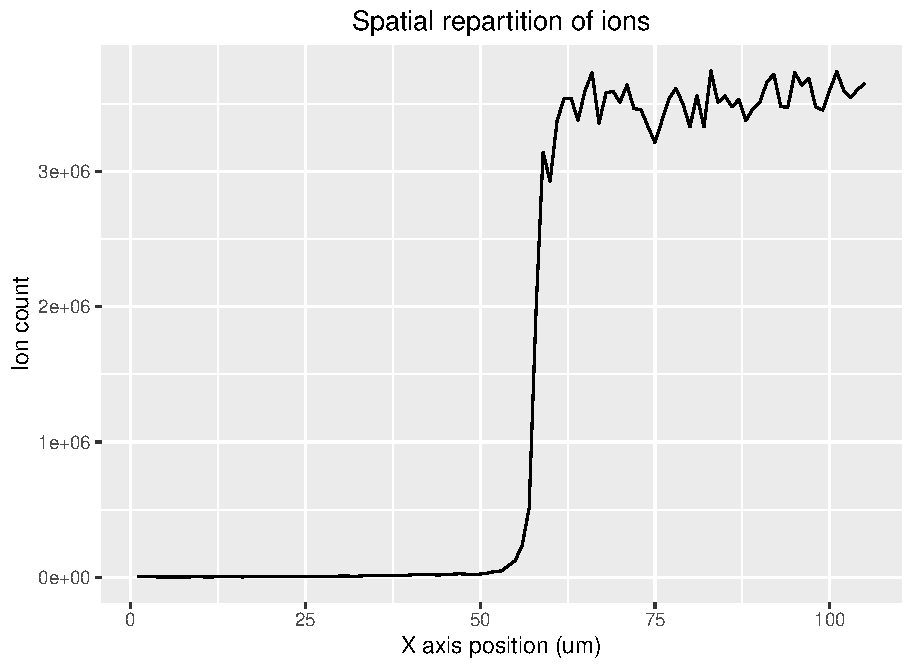
\includegraphics[scale = .5, keepaspectratio]{application/response_estimation/data_1d.pdf}
	\end{figure}
\end{column}
\end{columns}
\end{frame}

\begin{frame}{Noise estimation}{Spectra of data}
\begin{columns}
\begin{column}{8cm}
\begin{figure}[H]
		\label{edge_2d}\caption{Spectra of the data in 2D}
		\centering
    	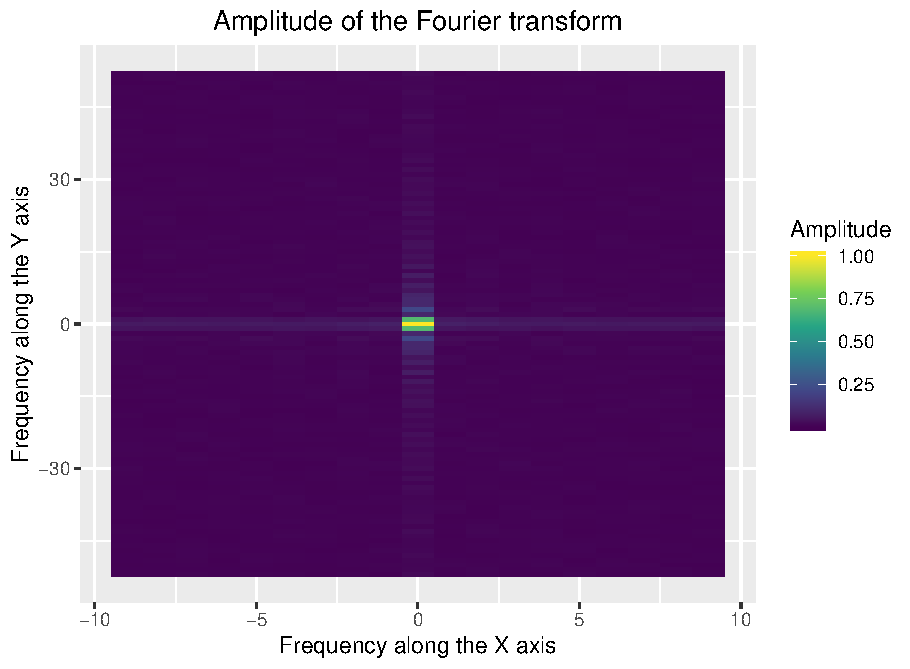
\includegraphics[scale = .5, keepaspectratio]{application/response_estimation/spectra_2d.pdf}
	\end{figure}
\end{column}
\begin{column}{8cm}
\begin{figure}[H]
		\label{edge_2d}\caption{Spectra of the data in 1D}
		\centering
    	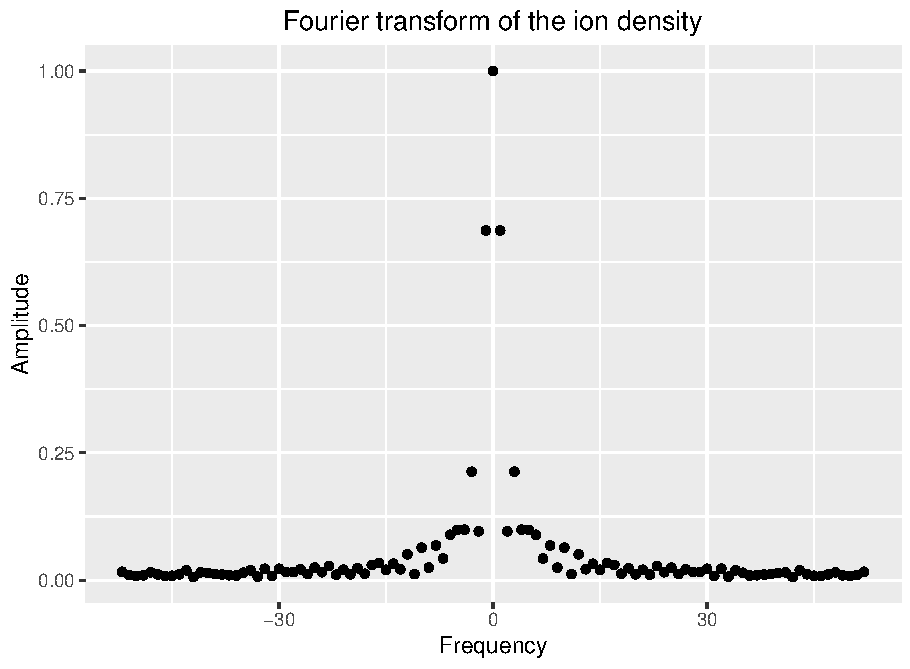
\includegraphics[scale = .5, keepaspectratio]{application/response_estimation/spectra_1d.pdf}
	\end{figure}
\end{column}
\end{columns}
\end{frame}

\begin{frame}{Noise estimation}{Adaptive smoothing as direct problem}
\begin{figure}[H]
		\label{edge_2d}\caption{Adaptive shrinkage estimator in 1D}
		\centering
    	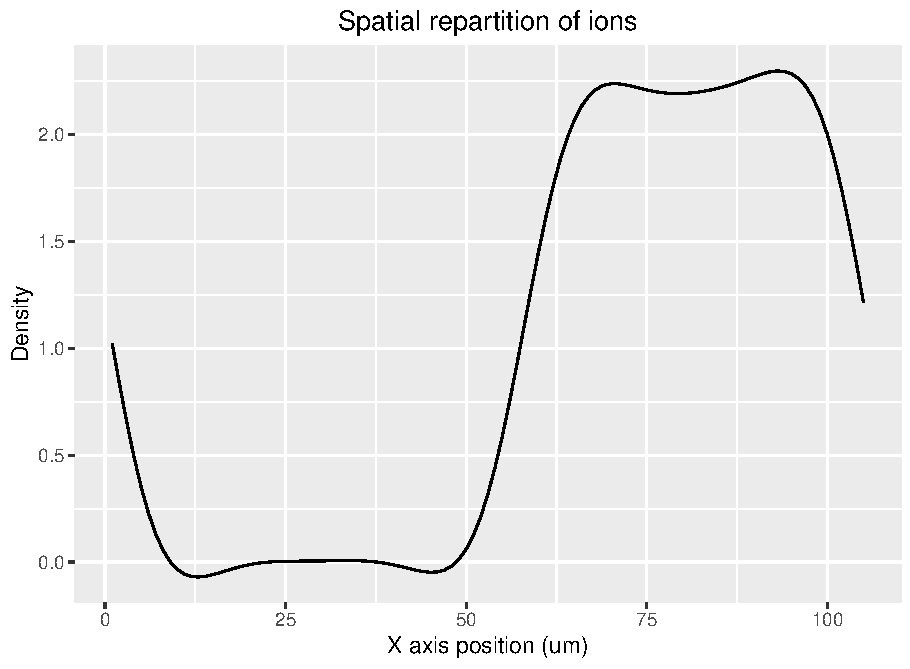
\includegraphics[scale = .5, keepaspectratio]{application/response_estimation/estim_direct_1d.pdf}
	\end{figure}
\end{frame}

\begin{frame}{Noise estimation}{Known distribution of molecules}
\begin{columns}
\begin{column}{8cm}
\begin{figure}[H]
		\label{edge_2d}\caption{Edge in 2D}
		\centering
    	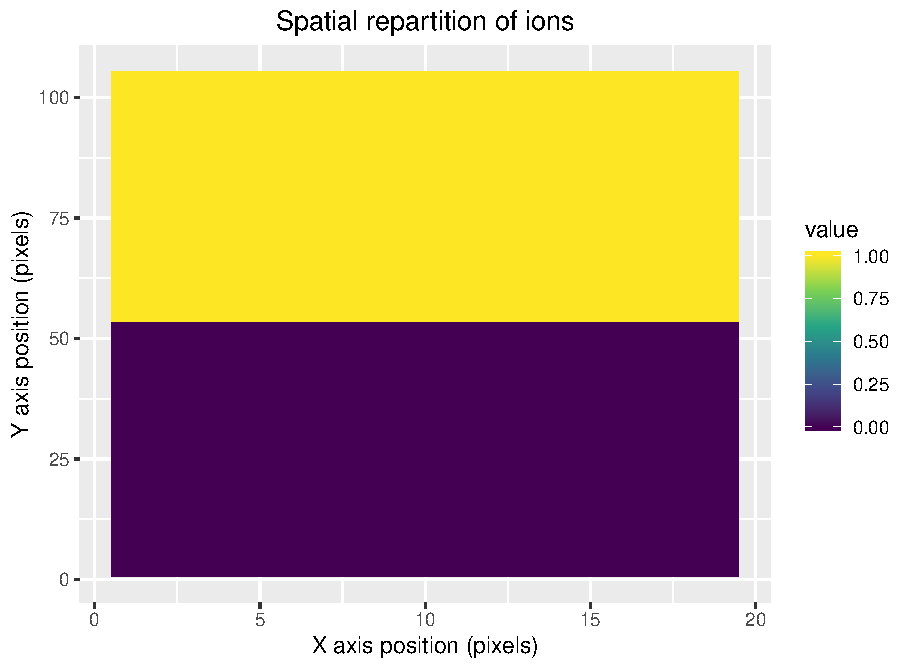
\includegraphics[scale = .5, keepaspectratio]{application/response_estimation/edge_2d.pdf}
	\end{figure}
\end{column}
\begin{column}{8cm}
\begin{figure}[H]
		\label{edge_1d}\caption{Edge in 1D}
		\centering
    	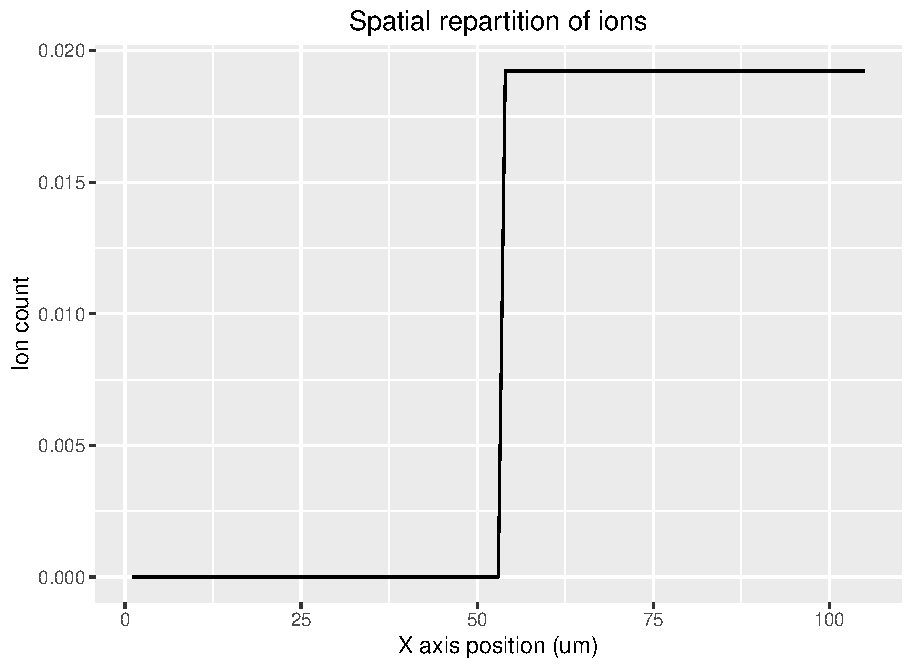
\includegraphics[scale = .5, keepaspectratio]{application/response_estimation/edge_1d.pdf}
	\end{figure}
\end{column}
\end{columns}
\end{frame}

\begin{frame}{Noise estimation}{Spectra of the edge}
\begin{columns}
\begin{column}{8cm}
\begin{figure}[H]
		\label{edge_2d}\caption{Spectra of the edge in 2D}
		\centering
    	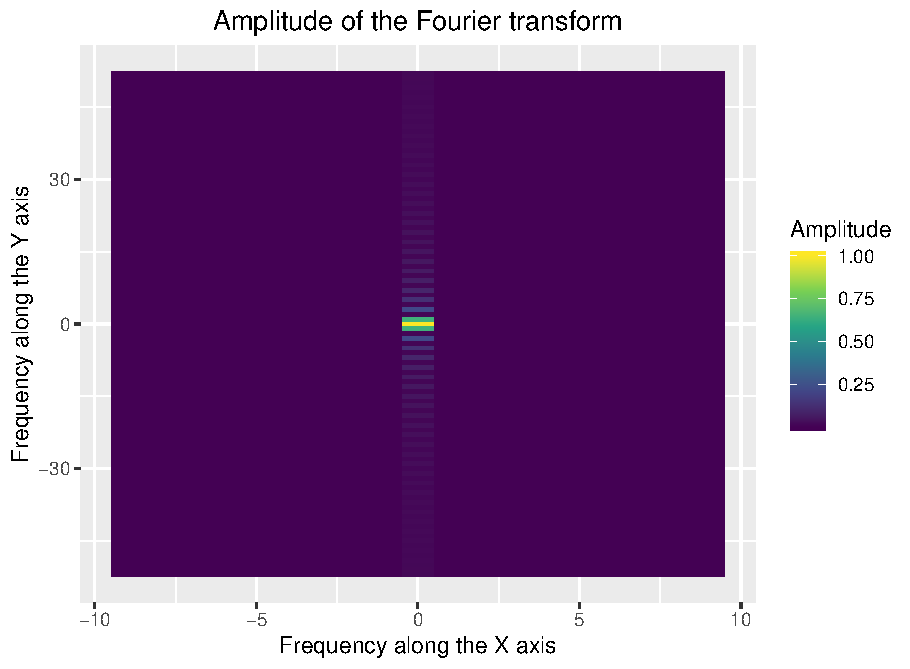
\includegraphics[scale = .5, keepaspectratio]{application/response_estimation/spectra_edge_2d.pdf}
	\end{figure}
\end{column}
\begin{column}{8cm}
\begin{figure}[H]
		\label{edge_2d}\caption{Spectra of the edge in 1D}
		\centering
    	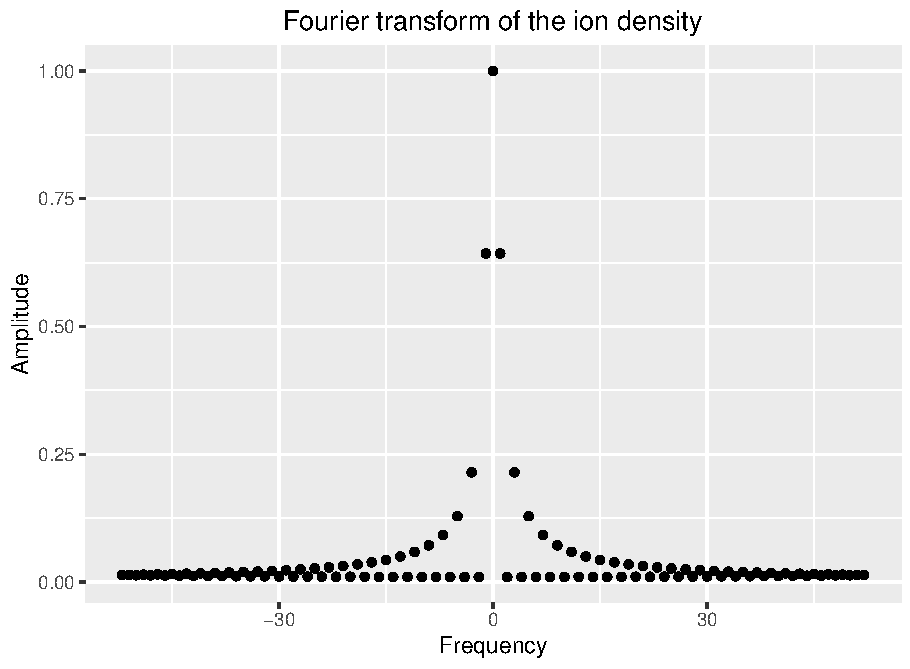
\includegraphics[scale = .5, keepaspectratio]{application/response_estimation/spectra_edge_1d.pdf}
	\end{figure}
\end{column}
\end{columns}
\end{frame}

\begin{frame}{Noise estimation}{Ionisation probability function estimate in 1D}
\begin{columns}
\begin{column}{8cm}
\begin{figure}[H]
		\label{edge_2d}\caption{Adaptive shrinkage estimator of $\mathcal{I}_{\mathds{P}}(t_{0}, \cdot)$ in 1D}
		\centering
    	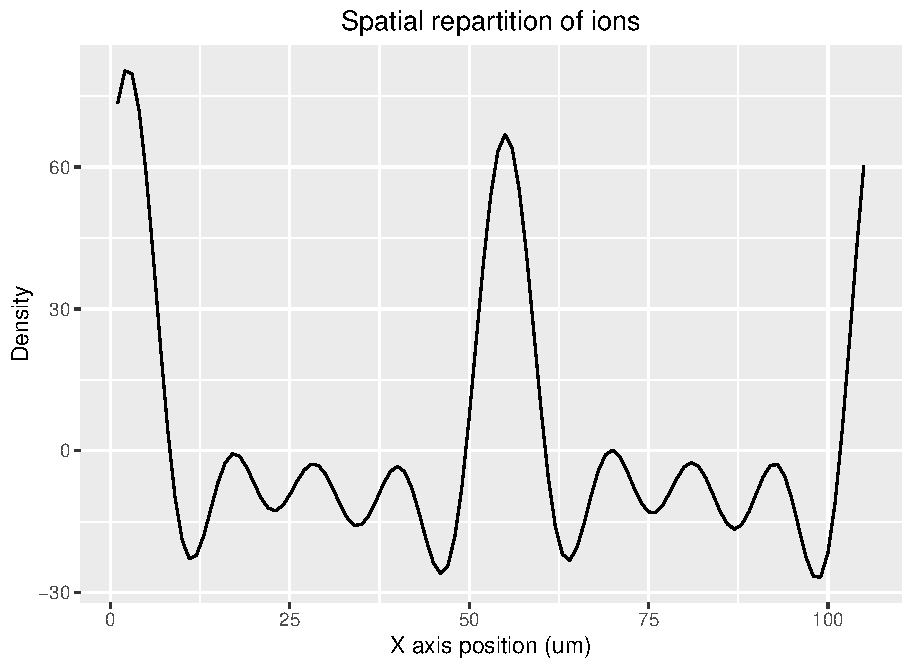
\includegraphics[scale = .5, keepaspectratio]{application/response_estimation/estim_noise_1d.pdf}
	\end{figure}
\end{column}
\begin{column}{8cm}
\begin{figure}[H]
		\label{edge_2d}\caption{Adaptive shrinkage estimator of $\mathcal{I}_{\mathds{P}}(t_{0}, \cdot)$ in 1D}
		\centering
    	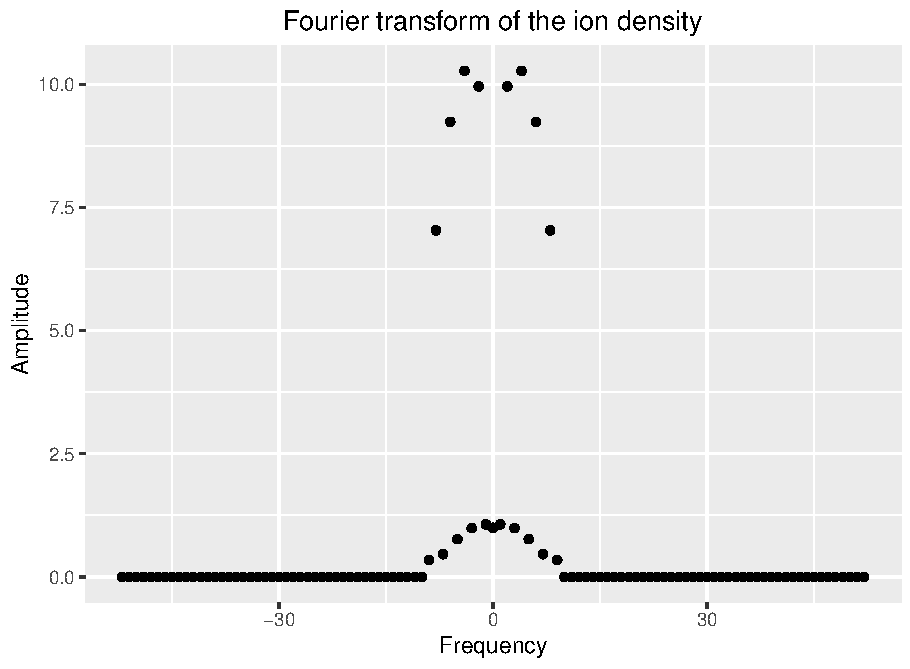
\includegraphics[scale = .5, keepaspectratio]{application/response_estimation/spectra_estim_noise_1d.pdf}
	\end{figure}
\end{column}
\end{columns}
\end{frame}

\begin{frame}{Noise estimation}{Progress in this direction}
\begin{itemize}
\item complete implementation in 2D;
\item estimate quantiles of $\mathcal{I}_{\mathds{P}}$;
\item confidence bands for $\mathcal{I}_{\mathds{P}}$;
\item far future (spatial statistic): from estimations of $\mathcal{I}_{\mathds{P}}$ for a set of parameters (time, laser profile, end-member nature,...) estimate it for new values of parameters.
\end{itemize}
\end{frame}